\section{$S= 3/2$ Thermometry}\label{spin1.5-thermo}
% \todo[inline, color=ediblue]{Check wrapfigs}

We consider again the V2 Silicon vacancy which due to the 4H-SiC trigonal
pyramidal symmetry has a stable ground state ZFS with respect to temperature and can not be used for thermometry \cite{Castelletto_2024}.
% However, the ZFS of the excited state of the Silicon vacancy has a much
% larger change rate with the temperature compared with the
% dD/dT of the ground state of the divacancy in 4H-SiC or the
% NV centre in diamond \cite{Anisimov2016}.

% This can be a promising tool for
% thermometry, although the change of the ZFS of the excited
% state can not be detected directly from the ODMR spectrum
% due to the short lifetime of the excited state. As discussed
% in the magnetometry section, in the vicinity of the LAC, the
% PL intensity reaches a local extreme point [28]. By adding a
Schemas have been developed which exploit the increase in photoluminescence in the vicinity of level anti-crossings to measure the change in the excited state $D$ as in the work by Anisimov et al.

We will focus instead on an alternative all optical method which exploits the dependence on temperature of the photoluminescence of the spin system.

Anti-Stokes excitation is a process in which the wavelength of the exciting photon is longer (i.e. lower energy) than that
of the emitted photons (visualised in figure \ref{fig:anti-stokes}).  The mechanisms of anti-stokes excitation have been studied and include multiphoton absorption, phonon absorption, and Auger recombination
\cite{Tran2019, Wang2019}.

\begin{wrapfigure}{l}{0.37\textwidth}%
	\centering%
	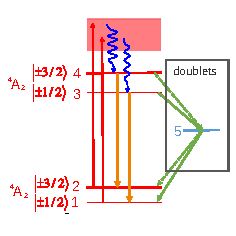
\includegraphics[width=0.37\textwidth]{figures/actual-stokes.pdf}
    \caption{Energy level diagram showing Stokes excitation. Colours as described in figure \ref{fig:big_stokes}. Adapted from Wang et al.}
    \label{fig:stokes}
	% \todo[inline, color=ediblue]{Write caption}
\end{wrapfigure}%



The anti-Stokes excitation process depends on a contribution from phonons (blue arrows in in figure \ref{fig:anti-stokes}).

By comparing the intensity of the anti-Stokes and Stokes photoluminescence we find the ratio between the intensities to be proportional to the phonon density, which are determined by a Bose–Einstenin distribution \cite{Wang2018}
\begin{equation}
	\frac{I_{\ce{AS}}}{I_{\ce{S}}} \propto \exp\left\{\frac{\Delta E}{k_B T} -1 \right\}
	\label{eq:anti-stoke-ratio}
\end{equation}
where $I_{\ce{AS}}$ and $I_{\ce{S}}$ represent respectively the intensities of the anti-Stokes and Stokes photoluminescence at a datum laser power. $\Delta E$ represents the difference in energy between the incident photon and the zero phonon line i.e. the phonon contribution to the excitation.

\begin{wrapfigure}{r}{0.4\textwidth}%
	\centering%
	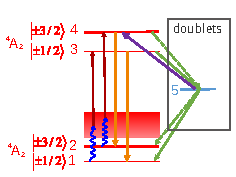
\includegraphics[width=0.4\textwidth]{figures/stokes.pdf}
    \caption{Energy level diagram showing anti-Stokes excitation. Colours as described in figure \ref{fig:big_stokes}. Adapted from Wang et al.}
    \label{fig:anti-stokes}
	% \todo[inline, color=ediblue]{Write caption}
\end{wrapfigure}%
% When ∆E ≫ kB T,
% we approximately have IASPL /IPL ∝ exp(−∆E/kB T) [165].

We may reduce this to a temperature dependent exponential curve when $\Delta E \ll k_B T$ as \eqref{eq:anti-stoke-ratio} reduces to
\begin{equation}
	\frac{I_{\ce{AS}}}{I_{\ce{S}}} \propto \exp\left\{\frac{\Delta E}{k_B T} \right\}.
	\label{eq:anti-stokes-ratio-reduced}
\end{equation}

Wang et al analysed the Silicon vacancy under anti-Stokes excitation \cite{Wang2021}. The zero phonon line for the defect is around $917$nm, so a Stokes excitation was induces by a laser with $1030 > 917$nm and the anti-Stokes excitation was induced by a laser with $720 < 917$nm. Using the same power for both lasers, the intensity of the photoluminescence from the anti-Stokes excitation increased as temperature increased. Conversely the intensity from the Stokes excitation decreased with temperature. The ratio therefore agrees with the statistical model in \eqref{eq:anti-stoke-ratio}.

Thus to realise a thermometer, we fit data to \eqref{eq:anti-stokes-ratio-reduced} with measurable proportionality and correction factors $a, b, c, T_0$ as \cite{Tran2019}
\begin{equation}
	\frac{I_{\ce{AS}}}{I_{\ce{S}}} = a +  b\exp\left\{-\frac{c}{T - T_0} \right\}.
	\label{eq:s1.5thermo_exponential}
\end{equation}

Temperature may then be inferred by solving the equation as
\begin{equation}
	T = T_0 - \frac{c}{\ln\left(\left[{\frac{I_{\ce{AS}}}{I_{\ce{S}}} - a}\right]/b\right)}.
	\label{eq:anti-stokes-solution}
\end{equation}

For the SiC Silicon vacancy the intensity ratio, and thus the proposed thermometry sensitivity, is most sensitive at room temperature and above.

This technique is also extremely versatile as the influence of external parameters, providing they do not change the position of the zero phonon line (effect ZFS $D$), does not affect the measurement. For example, figure \ref{fig:anti-stokes-ODMR} shows that the ODMR signature which can be used to detect magnetic field can be read in parallel to the ratio of intensities of the Stokes/anti-Stokes excitations. We will discuss how this may be applied in Chapter \ref{ch:results}.



\begin{figure}[h]
	\centering
	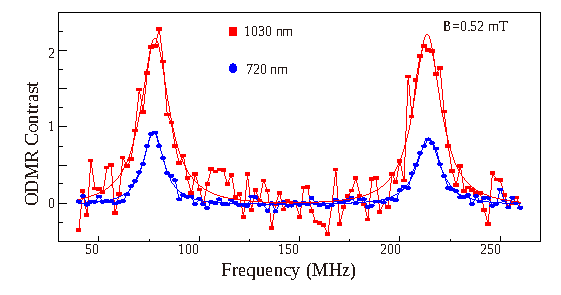
\includegraphics[width=0.8\textwidth]{figures/anti-stokes-ODMR.pdf}
	\caption{ODMR spectra for V2 Silicon vacancy using Stokes (blue) and anti-Stokes (red) excitation. This shows the Rabi frequencies are the same under either excitation scheme. Adapted from Wang et al}
    \label{fig:anti-stokes-ODMR}
	% Stokes
	% (blue) and AS excited (red) ODMR spectra of VSi defects for the same Rabi frequency (0.8 MHz) at different c-axis external magnetic fields
\end{figure}



% \todo[color=red, inline]{Affects of other factors? e.g. $\vec{B}, \vec{E}$}


% \begin{figure}[H]
%     \begin{center}
%         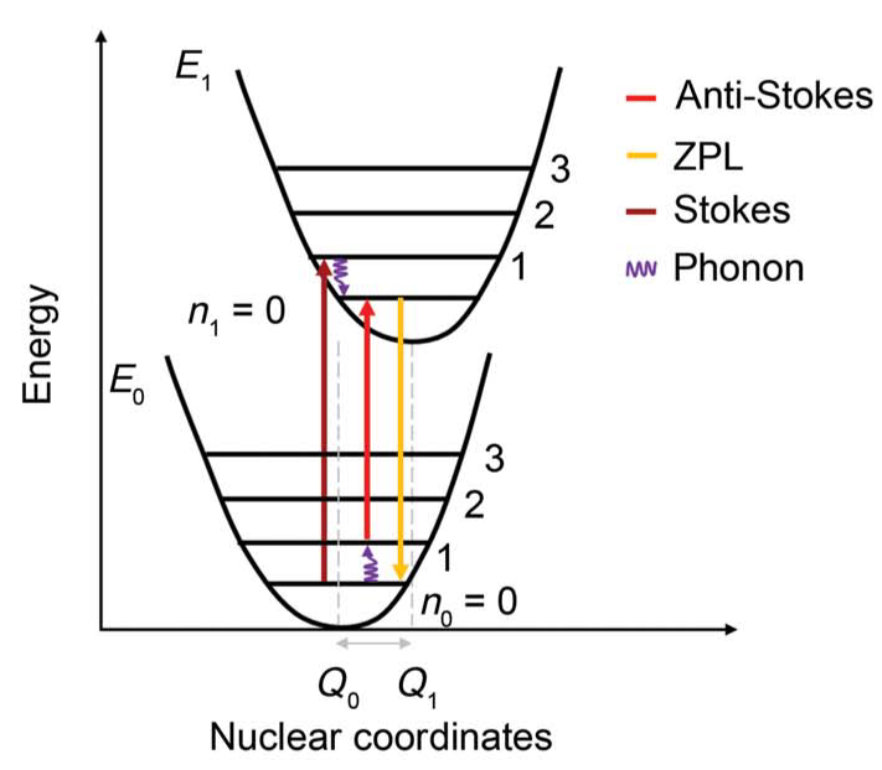
\includegraphics[width=0.4\textwidth]{figures/stokes.png}
%     \end{center}
%     \caption{}\label{fig:stokes}
% \end{figure}


\begin{summary}{$S=3/2$ Thermometry Summary}{sum:spin1.5thermo}
	We may achieve optical thermometry using an $S = 3/2$ system provided:
	\begin{enumerate}
		\item The ZFS parameters $D$ and $E$ are well known and we may determine the position of the zero phonon line.
		\item The system is responsive to both Stokes and anti-Stokes excitation and the intensities of the subsequent emission can be measured.
		\item The temperature dependence of the ratio between intensities has been studied and mapped to an exponential equation as             \begin{equation}
			      \tcbhighmath{
				      \frac{I_{\ce{AS}}}{I_{\ce{S}}} = a +  b\exp\left\{-\frac{c}{T - T_0} \right\},
			      }
			      \tag{\ref{eq:s1.5thermo_exponential}}
		      \end{equation}
		      from which the temperature can be calculated as
            \begin{equation}
			      \tcbhighmath{
				      T = T_0 - \frac{c}{\ln\left(\left[{\frac{I_{\ce{AS}}}{I_{\ce{S}}} - a}\right]/b\right)}.
			      }
			      \tag{\ref{eq:anti-stokes-solution}}
		      \end{equation}


	\end{enumerate}
\end{summary}

